% Figure snippets for main.tex. Embedded inline by the writing agent.

\begin{figure}[htbp]
\centering
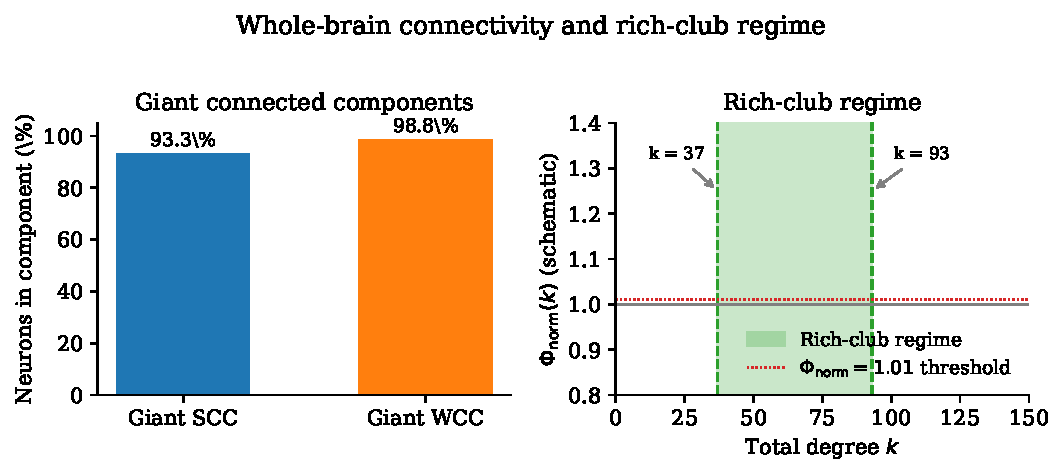
\includegraphics[width=0.95\linewidth]{figures/fig1_global.pdf}
\caption{Whole-brain connectivity and rich-club regime.
(a) Fraction of the 127{,}978 neurons contained in the giant strongly connected
component (SCC; 93.3\%) and in the giant weakly connected component (WCC;
98.8\%) after thresholding at five synapses per connection.
(b) The rich-club regime lies between total-degree $k=37$ and $k=93$, the range
over which the normalized rich-club coefficient $\Phi_{\mathrm{norm}}(k)$
exceeds the $1.01$ threshold relative to 100 configuration null models.}
\label{fig:global}
\end{figure}

\begin{figure}[htbp]
\centering
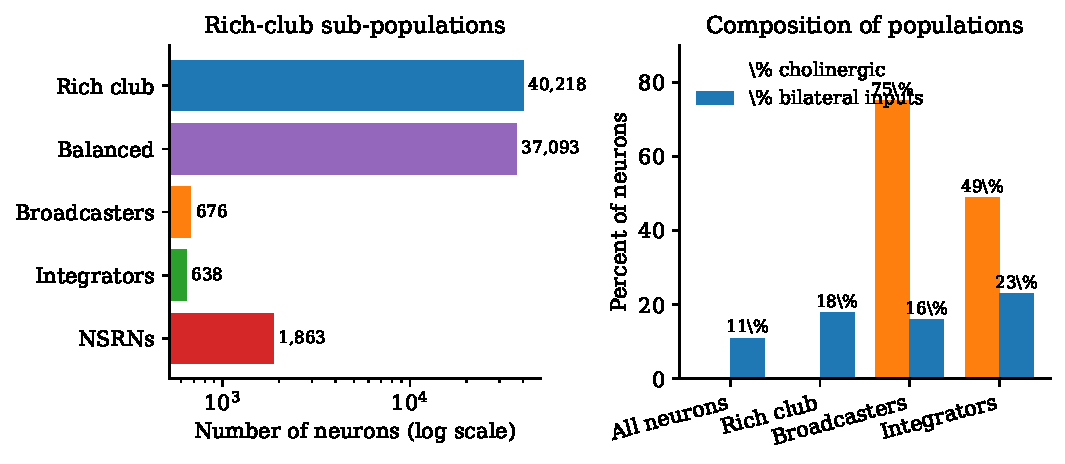
\includegraphics[width=0.95\linewidth]{figures/fig2_populations.pdf}
\caption{Rich-club sub-populations identified in the FlyWire connectome.
(a) Neuron counts for the rich-club ($n=40{,}218$), balanced ($n=37{,}093$),
broadcaster ($n=676$), integrator ($n=638$), and neuropil-specific highly
reciprocal neuron (NSRN; $n=1{,}863$) populations.
(b) Cholinergic fraction (where reported) and fraction of neurons with inputs
in both hemispheres. Broadcasters are 75\% cholinergic; integrators are 49\%
cholinergic. Bilateral inputs: 11\% of all neurons, 18\% of rich-club neurons,
16\% of broadcasters, 23\% of integrators.}
\label{fig:populations}
\end{figure}

\begin{figure}[htbp]
\centering
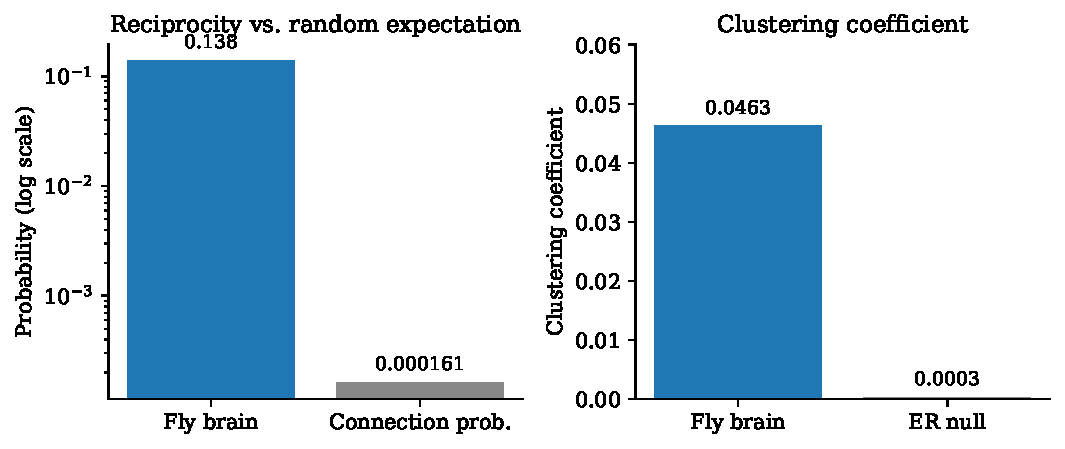
\includegraphics[width=0.9\linewidth]{figures/fig3_recip_clustering.pdf}
\caption{Reciprocity and clustering in the fly brain against random baselines.
(a) Whole-brain reciprocity is $0.138$, much larger than the global
connection probability of $0.000161$ that would set the baseline for an
undirected random pairing.
(b) The global clustering coefficient of the fly brain ($0.0463$) is two
orders of magnitude larger than the value expected under a matched directed
Erd{\H o}s--R{\'e}nyi null model ($0.0003$).}
\label{fig:recip}
\end{figure}

\begin{figure}[htbp]
\centering
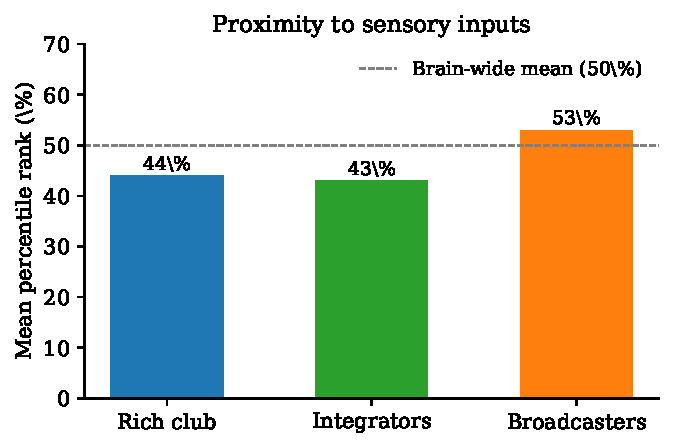
\includegraphics[width=0.6\linewidth]{figures/fig4_sensory_rank.pdf}
\caption{Mean percentile rank of rich-club sub-populations relative to the
complete set of sensory inputs under the probabilistic information-flow
model of Schlegel and colleagues. Rich-club neurons (44\%) and integrators
(43\%) are on average closer to sensory inputs than the brain-wide mean
(50\%), whereas broadcasters (53\%) are slightly farther.}
\label{fig:rank}
\end{figure}
